\documentclass[10pt,a4paper]{article}
\usepackage[natbibapa]{apacite} 
\usepackage{amsmath}
\usepackage{tikz}

\bibliographystyle{apacite}

\tikzset{
  treenode/.style = {shape=rectangle, rounded corners,
                     draw, align=center,
                     top color=white, bottom color=blue!20},
  root/.style     = {treenode, font=\Large, bottom color=red!30},
  env/.style      = {treenode, font=\ttfamily\normalsize},
  dummy/.style    = {circle,draw}
}

\title{Assignment 1}
\author{ Adriaan Louw (53031377)}

\begin{document}

\maketitle

\tableofcontents

\section{Question 1}

The book \emph{Introduction to Machine Learning} by Nils J, Nilsson can be found at
http://robotics.stanford.edu/people/nilsson/MLBOOK.pdf and is 1.855 MB.

The book \emph{A first encounter with Machine Learning} by Max Welling can be found at 
http://citeseerx.ist.psu.edu/viewdoc/download?doi=10.1.1.441.6238\&rep=rep1\&
type=pdf and is 416 KB.

\section{Question 2}

We can represent some learning functions in machine learning as Boolean function. We can define a Boolean function as a function of the form

\begin{equation}
f(x_1,x_2,x_3,...x_n)
\end{equation}

Which maps a n-tuple of (0,1) values to {0,1}. {0,1} can also be expressed as {false,true}.

There are 3 basic types of operations can be performed in Boolean functions. Firstly we have the "and" operation which uses the connective "." as in

\begin{equation}
x_1.z_2
\end{equation}

Which only returns true if $x_1$ and $x_2$ is true. Then there is the "or" operation represented as a "+"

\begin{equation}
x_1+x_2
\end{equation}

Where it returns true if $x_1$ is true or if $x_2$ or both are true. Thirdly we have the negation operation indicated by a $\bar{}$ as in 

\begin{equation}
\bar{x_1}
\end{equation}

This operation returns true if $x_1$ is false and false if $x_1$ is true.

The . and + operations are commutative 

\begin{equation}
\begin{split}
x_1.x_2 &= x_2.x_1 \\
x_1+x_2 &= x_2 + x_1 \\
\end{split}
\end{equation}

and associative

\begin{equation}
\begin{split}
x_1.x_2(x_3) &= x_1(x_2.x_3) \\
x_1 + x_2 + ( x_3 ) &= x_1 + ( x_2 + x_3 ) \\
\end{split}
\end{equation}

To commute between . and + we use DeMorgan's laws

\begin{equation}
\begin{split}
\overline{x_1.x_2} &= \overline{x_1} + \overline{x_2} \\
\overline{x_1 + x_2} &= \overline{x_1}.\overline{x_2} \\
\end{split}
\end{equation}

Boolean functions can be broken down into various sub-classes. The first subclass is called \emph{terms}. We can write these as $k_1k_2k_3...k_n$ where $k_i$ are literals. An example would be the following term of size 4, $x_2.x3.\overline{x_6}.x_{12}$. This is also called a conjunctive literal as in all the terms  are separated by the and operation.

Secondly we have \emph{clauses} or . A clause is a function where the literals are separated by the or function. As in $k_1+k_2 + ... + k_n $. An example would be $x_1 + \overline{x_5} + x_8$.

Disjunctive normal functions are functions that can be written as a disjunction of terms. 








\section{Question 3}
\section{Question 4}
\section{Question 5}
\subsection{Question 5.1}
$A\wedge B$

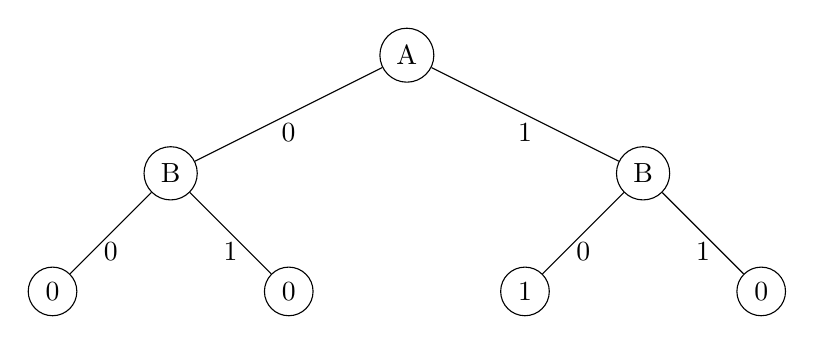
\begin{tikzpicture}
 [level/.style={sibling distance=60mm/#1}]
 
  \node [circle,draw] {A}
    child { node [circle,draw] {B}
      child { node[dummy] {0}
         edge from parent node [below] {0} }
      child { node[dummy] {0}
         edge from parent node [below] {1} }    
      edge from parent node[below] {0} }
    child { node [circle,draw] {B}
      child { node [dummy] {1}
        edge from parent node [below] {0} } 
      child { node [dummy] {0}
         edge from parent node [below] {1} }  
      edge from parent node[below] {1}};
\end{tikzpicture}



\section{Question 6}

Entropy is used to calculate a decision tree in the ID3 algorithm. For a collection of Samples ($S$):

\begin{equation}
\label{ent}
Entropy(S) = \sum_{i=1}^c -p_i log_2p_i
\end{equation}

If we assume we only have 2 outcomes, then we let the number of positive outcomes by p and the number of negative outcomes be n. Then we can write Equation \ref{ent} as

\begin{equation}
Entropy(p,n) = -\frac{p}{p+n}log_2\frac{p}{p+n} - \frac{n}{p+n}log_2\frac{n}{p+n} 
\end{equation}
 
More specifically we compare the gain of different attributes of the sample set. Then create the tree based on the attributes with the greatest gain

\begin{equation}
Gain(S,A) \equiv Entropy(S) - \sum_{v \in Values(A)} \frac{\vert S_v\vert}{\vert S\vert}Entropy(S_v)
\end{equation}

We need to determine $Entropy(S)$

\begin{equation}
\begin{split}
Entropy(p,n) &=  -\frac{p}{p+n}log_2\frac{p}{p+n} - \frac{n}{p+n}log_2\frac{n}{p+n}  \\
           &= -\frac{3}{3+1} log_2\frac{3}{3+1} -\frac{1}{3+1} log_2\frac{1}{3+1} \\
           &=    \\
\end{split}
\end{equation}

Now we need to determine the gain for the 6 attributes to determine which one will be the root node.

For Sky we have sunny {$p_1=3,n_1=0$) and rainy {$p_1=0,n_1=1$)
\begin{equation}
\begin{split}
Gain(S,Sky) &= Entropy(S) - \sum_{v \in Values(A)} \frac{\vert S_v\vert}{\vert S\vert}Entropy(S_v) \\
          &= ?? - \frac{1}{4} Entropy(S_{Sunny} ) - Entropy(S_{Rainy}) \\
          &= ?? - \frac{1}{4} Entropy(3,0) - Entropy(0,1) \\
          &= ?? -\frac{3}{4} ( -\frac{3}{3} log_2\frac{3}{3} -\frac{0}{3} log_2\frac{0}{3} ) - \frac{1}{4}(-\frac{0}{1} log_2\frac{0}{1} - \frac{1}{1}log_2\frac{1}{1} ) \\
          &= 
\end{split}
\end{equation}


\bibliography{mybib}
\end{document}
